\newpage
\phantomsection
\addcontentsline{toc}{chapter}{ANEXOS}
\setcounter{section}{0}
\renewcommand{\thesection}{\Alph{section}}
\renewcommand{\theHsection}{appendixsection.\Alph{section}}

\chapter*{ANEXOS}
\section*{ANEXO A - ÁRBOL DE PROBLEMAS}
\begin{center}
%    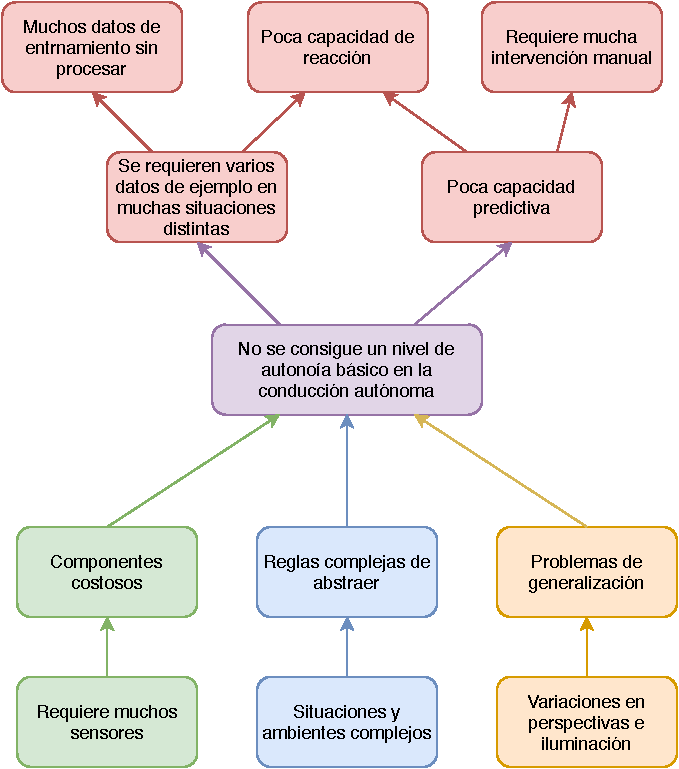
\includegraphics[scale=0.56]{imagenes/arbol_de_problemas}
	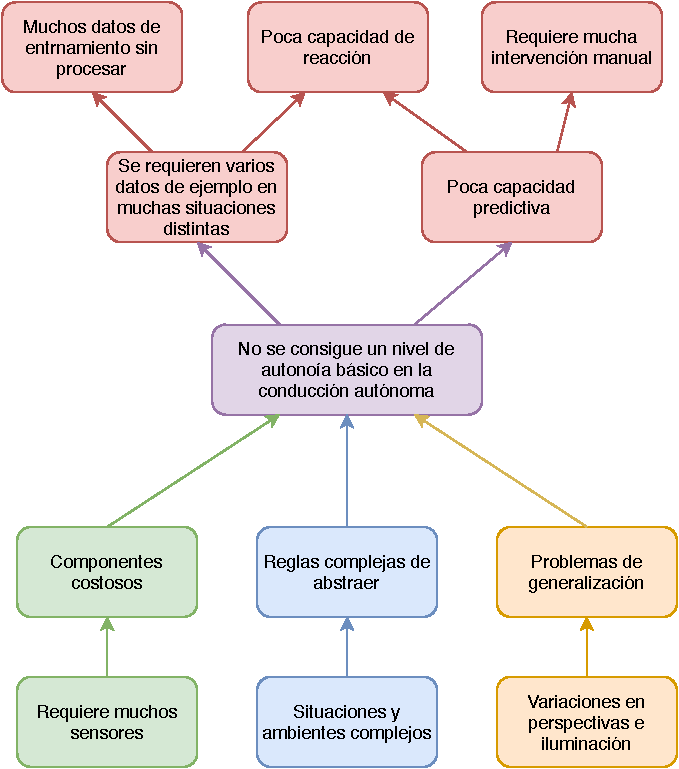
\includegraphics[scale=1]{imagenes/arbol_de_problemas}
\end{center}
\newpage
\section*{ANEXO B - ÁRBOL DE OBJETIVOS}
\begin{center}
%    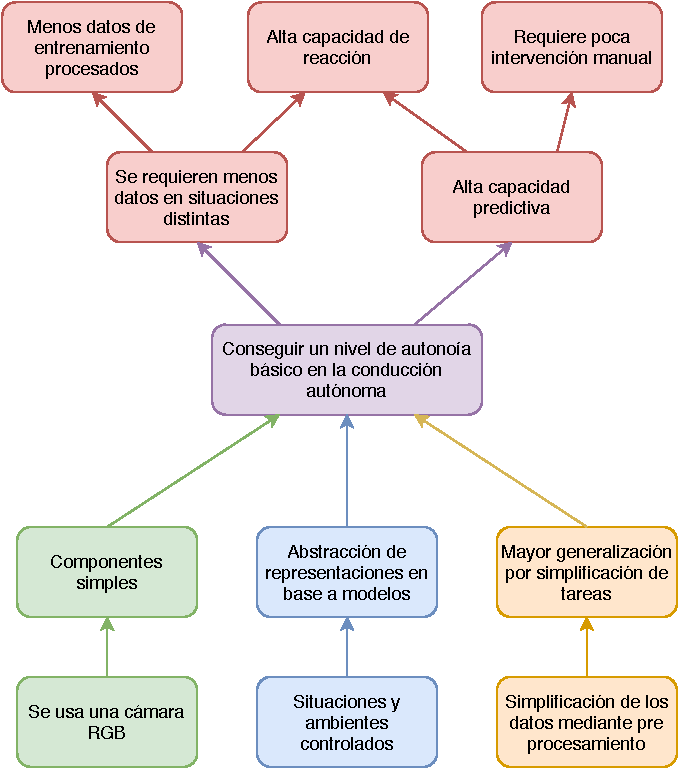
\includegraphics[scale=0.56]{imagenes/arbol_de_objetivos}
	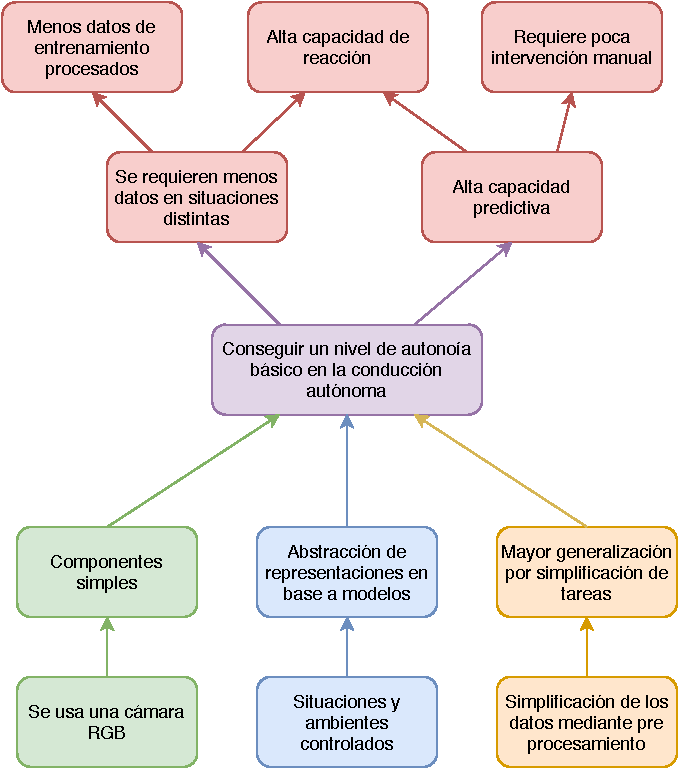
\includegraphics[scale=1]{imagenes/arbol_de_objetivos}
\end{center}
\newpage
\section*{ANEXO C - MARCO LÓGICO}
\begin{center}
%    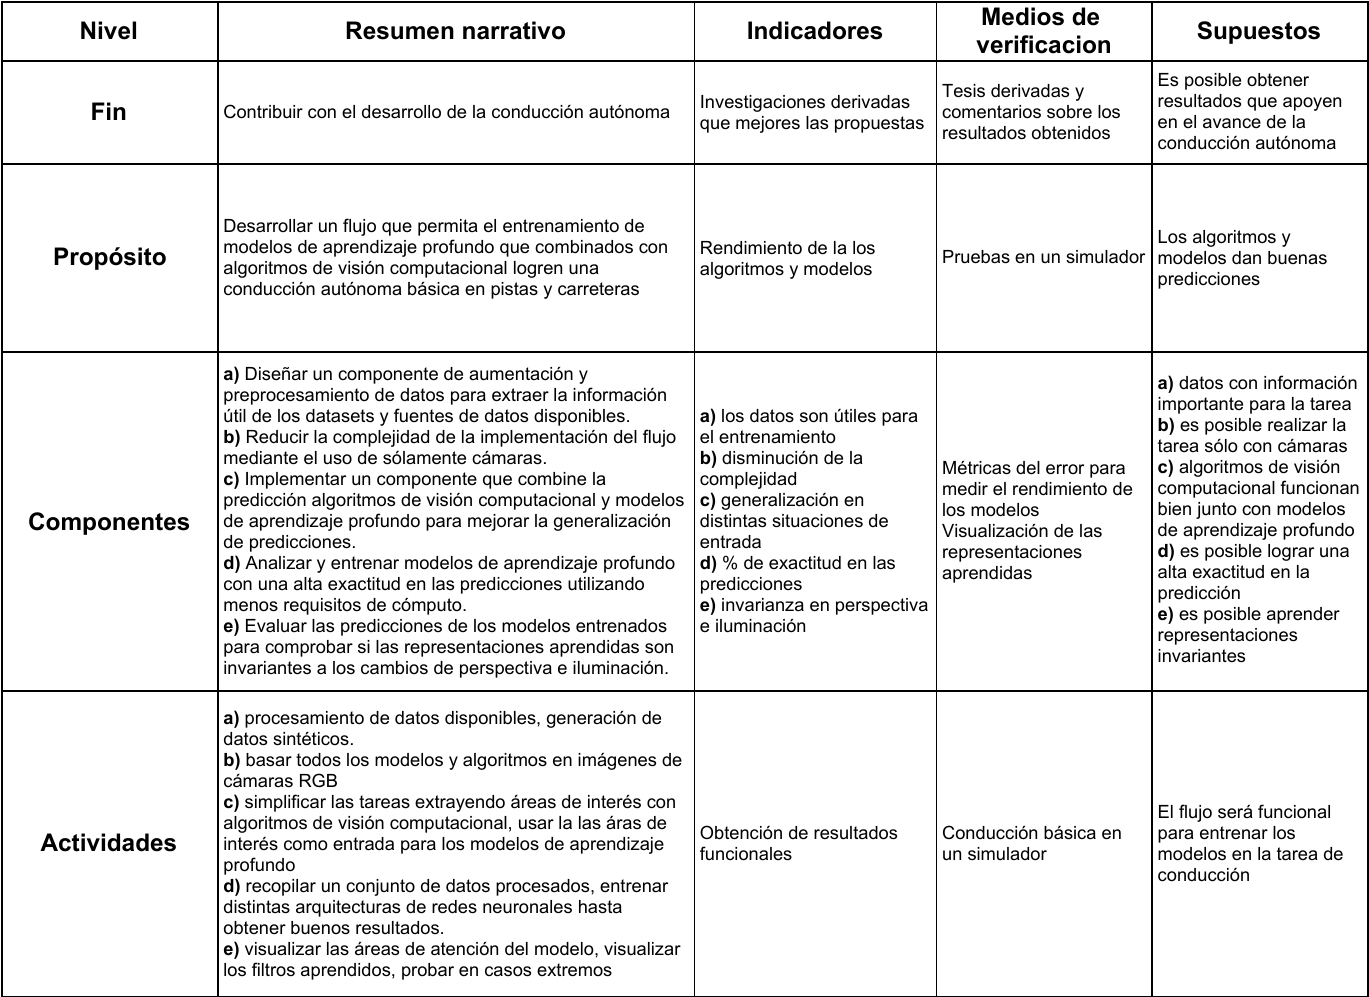
\includegraphics[scale=0.34]{imagenes/marco_logico-1}
    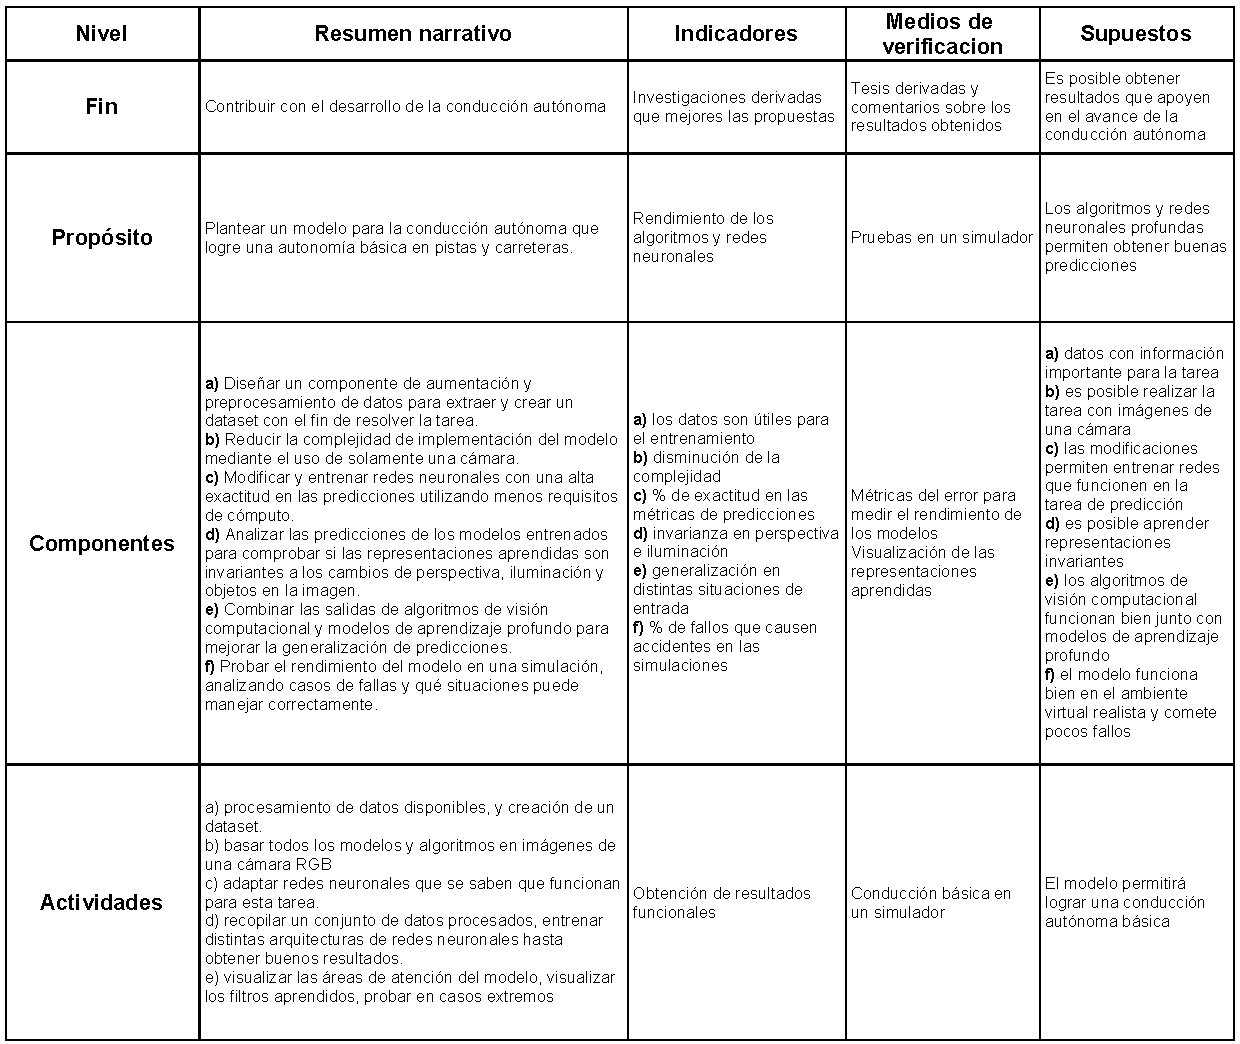
\includegraphics[scale=0.8]{imagenes/MarcoLogico}
\end{center}
\newpage

% Preparación de Datos
% Extracción de imagenes
% Unificar df
% Preparación de intersecciones en carpetas
% Unificar df con juncs
\section*{ANEXO D - PREPARACIÓN DE DATOS}
\subsection*{D.1 - EXTRACCIÓN DE IMÁGENES}
	\inputminted[frame=lines,
	baselinestretch=1,
	fontsize=\footnotesize,
	autogobble]{python}{codigos/apendices/extraccion.py}
\subsection*{D.2 - UNIFICACIÓN DE LOS DATAFRAMES}
	\inputminted[frame=lines,
	baselinestretch=1,
	fontsize=\footnotesize,
	autogobble]{python}{codigos/apendices/unificar_df.py}
\subsection*{D.3 - PREPARACIÓN DE INTERSECCIONES}
	\inputminted[frame=lines,
	baselinestretch=1,
	fontsize=\footnotesize,
	autogobble]{python}{codigos/apendices/juncs.py}
\subsection*{D.4 - CREACIÓN DEL DATAFRAME FINAL}
	\inputminted[frame=lines,
	baselinestretch=1,
	fontsize=\footnotesize,
	autogobble]{python}{codigos/apendices/unificar_df_junc.py}
% Entrenamiento
	% Script de entrenamiento DriveNet
	% Script de entrenamiento DepthNet
	% Script de entrenamiento SemsegNet
\section*{ANEXO E - ENTRENAMIENTO DE REDES}
\subsection*{E.1 - DRIVENET}
	\inputminted[frame=lines,
	baselinestretch=1,
	fontsize=\footnotesize,
	autogobble]{python}{codigos/apendices/drive_train.py}
\subsection*{E.2 - DEPTHNET}
	\inputminted[frame=lines,
	baselinestretch=1,
	fontsize=\footnotesize,
	autogobble]{python}{codigos/apendices/depth_train.py}
\subsection*{E.3 - SEMSEGNET}
	\inputminted[frame=lines,
	baselinestretch=1,
	fontsize=\footnotesize,
	autogobble]{python}{codigos/apendices/semseg_train.py}
% Inferencia
	% Cola de prioridad
\section*{ANEXO F - INFERENCIA}
\subsection*{F.1 - COLA DE PRIORIDAD}
	\inputminted[frame=lines,
	baselinestretch=1,
	fontsize=\footnotesize,
	autogobble]{python}{codigos/apendices/priority_queue.py}
\subsection*{F.2 - CONSTANTES DE IMPLEMENTACIÓN}
	\inputminted[frame=lines,
	baselinestretch=1,
	fontsize=\footnotesize,
	autogobble]{python}{codigos/apendice_d/constants.py}
\section*{F.3 - IMPLEMENTACIÓN DEL MODELO}
	\inputminted[frame=lines,
	baselinestretch=1,
	fontsize=\footnotesize,
	autogobble]{python}{codigos/apendice_e/inferencia.py}
	
\section*{ANEXO G - Repositorio de Código}
	\href{https://github.com/nubol23/sdc-bsc-thesis}{Enlace al repositorio de código en GitHub: https://github.com/nubol23/sdc-bsc-thesis}

% \footnotesize
% {\setstretch{1.0}
% \begin{center}
%     \begin{tabularx}{\textwidth}{|l|X|X|X|X|}
%         \hline
%         Nivel &	Resumen narrativo &	Indicadores & Medios de verificacion & Supuestos\\
%         \hline
%         Fin & Contribuir con el desarrollo de la conducción autónoma & Investigaciones derivadas que mejores las propuestas &	Tesis derivadas y comentarios sobre los resultados obtenidos &	Es posible obtener resultados que apoyen en el avance de la conducción autónoma\\
%         \hline
%         Propósito & Desarrollar un flujo que permita el entrenamiento de modelos de aprendizaje profundo que combinados con algoritmos de visión computacional logren una conducción autónoma básica en pistas y carreterasDesarrollar un flujo que permita el entrenamiento de modelos de aprendizaje profundo que combinados con algoritmos de visión computacional logren una conducción autónoma básica en pistas y carreteras & Rendimiento de la los algoritmos y modelos & Pruebas en un simulador & Los algoritmos y modelos dan buenas predicciones\\
%         \hline
%         Componentes & 
%         \begin{itemize}[nosep]
%             \item Diseñar un componente de aumentación y preprocesamiento de datos para extraer la información útil de los datasets y fuentes de datos disponibles.
%             \item Reducir la complejidad de la implementación del flujo mediante el uso de sólamente cámaras.
%             \item Implementar un componente que combine la predicción algoritmos de visión computacional y modelos de aprendizaje profundo para mejorar la generalización de predicciones.
%             \item Analizar y entrenar modelos de aprendizaje profundo con una alta exactitud en las predicciones utilizando menos requisitos de cómputo.
%             \item Evaluar las predicciones de los modelos entrenados para comprobar si las representaciones aprendidas son invariantes a los cambios de perspectiva e iluminación.
%         \end{itemize} & 
%         \begin{itemize}[nosep]
%             \item los datos son útiles para el entrenamiento
%             \item disminución de la complejidad
%             \item generalización en distintas situaciones de entrada
%             \item \% de exactitud en las predicciones
%             \item invarianza en perspectiva e iluminación
%         \end{itemize} & 
%         "Métricas del error para medir el rendimiento de los modelos
% Visualización de las representaciones aprendidas" &
%         \begin{itemize}[nosep]
%             \item datos con información importante para la tarea
%             \item es posible realizar la tarea sólo con cámaras
%             \item algoritmos de visión computacional funcionan bien junto con modelos de aprendizaje profundo
%             \item es posible lograr una alta exactitud en la predicción
%             \item es posible aprender representaciones invariantes
%         \end{itemize}\\
%         \hline
%     \end{tabularx}\\
% \end{center}
% }